\section{El arnés de experimentación}
\label{sec:annex-experiment-harness}

Este apéndice documenta la maquinaria detrás de la Sección~\ref{sec:empirical-evaluation}. Su propósito es la reproducibilidad entre rondas: un experimento nuevo es simplemente una carpeta nueva bajo \texttt{experimentos/}, y los mismos scripts de consolidación, reporte y publicación operan sobre ella sin cambios. El arnés está deliberadamente desacoplado del código del modelo en ambas direcciones---solo lee lo que entrenamiento y despliegue escriben---, de modo que un experimento nunca depende de la versión de la biblioteca que lo produjo y la biblioteca nunca se entera de la campaña que la usó. La consecuencia práctica es que las rondas siguen siendo interpretables y reconstruibles mucho después de que la biblioteca haya evolucionado.

\subsection{Etapas y registros}

Cada configuración es un archivo YAML y un slug. El slug es un identificador corto que codifica la familia y los mezcladores: \texttt{attn\_nsa\_\_engram} es un par híbrido (primer mezclador \texttt{nsa}, segundo mezclador \texttt{engram}), \texttt{attn\_single\_mamba} es una línea base de un solo mezclador, y las familias de ablación llevan sus propios prefijos (\texttt{opt\_}, \texttt{norm\_}, \texttt{pe\_}, \texttt{trans\_}, \texttt{vit\_}, \texttt{task\_}, \texttt{tokenizer\_}, \texttt{batch\_}, \texttt{realdata\_}, \texttt{audio\_}, \texttt{bitnet\_}). Todas las corridas ejecutan las mismas cinco etapas: entrenar, exportar el checkpoint, desplegar en formato estándar y cuantizado, evaluar cuatro consignas enmascaradas reservadas por formato y exportar el paquete de Hugging Face.

La política de fallos merece una nota. Un fallo en una etapa se registra, no aborta la tanda y aparece después como una fila ausente en lugar de como un cero silencioso. La distinción importa para la estadística posterior: un modelo que falló al entrenar no debe confundirse con un modelo que entrenó y puntuó cero, y una celda ausente del atlas debe poder rastrearse hasta un fallo registrado y no hasta un hueco inadvertido.

Tres registradores escriben de forma independiente y se unen solo al momento del reporte:

\begin{enumerate}[leftmargin=*]
    \item \textbf{El log de entrenamiento paso a paso.} Un CSV por corrida con una fila por paso de optimización: pérdida, precisión, learning rate, normas de gradiente por grupo de parámetros, razón de recorte, tiempo por paso y rendimiento. La ronda~2 registró 2{,}656{,}372 filas, que se procesan en streaming y se reducen a medias por época antes de dibujar cualquier gráfico: nadie grafica 2,6 millones de puntos, y la reducción es determinista, así que la curva publicada es una función exacta del log crudo.
    \item \textbf{El censo de parámetros.} Para cada configuración, el número de parámetros de cada grupo de módulos (atención, embeddings, FFN, cabeza, normalización, codificación posicional, mHC, router, residual). Es lo que separa ``el modelo es más grande'' de ``el bloque de atención es más grande'' y permite atribuir el coste por componente y no solo por modelo.
    \item \textbf{El libro del pipeline.} Una fila por ejecución de etapa con categoría, estado, duración y código de retorno. Es el único registro de los fallos y, por tanto, la única fuente del análisis de fiabilidad.
\end{enumerate}

\begin{figure}[tbp]
\centering
\fitfigure{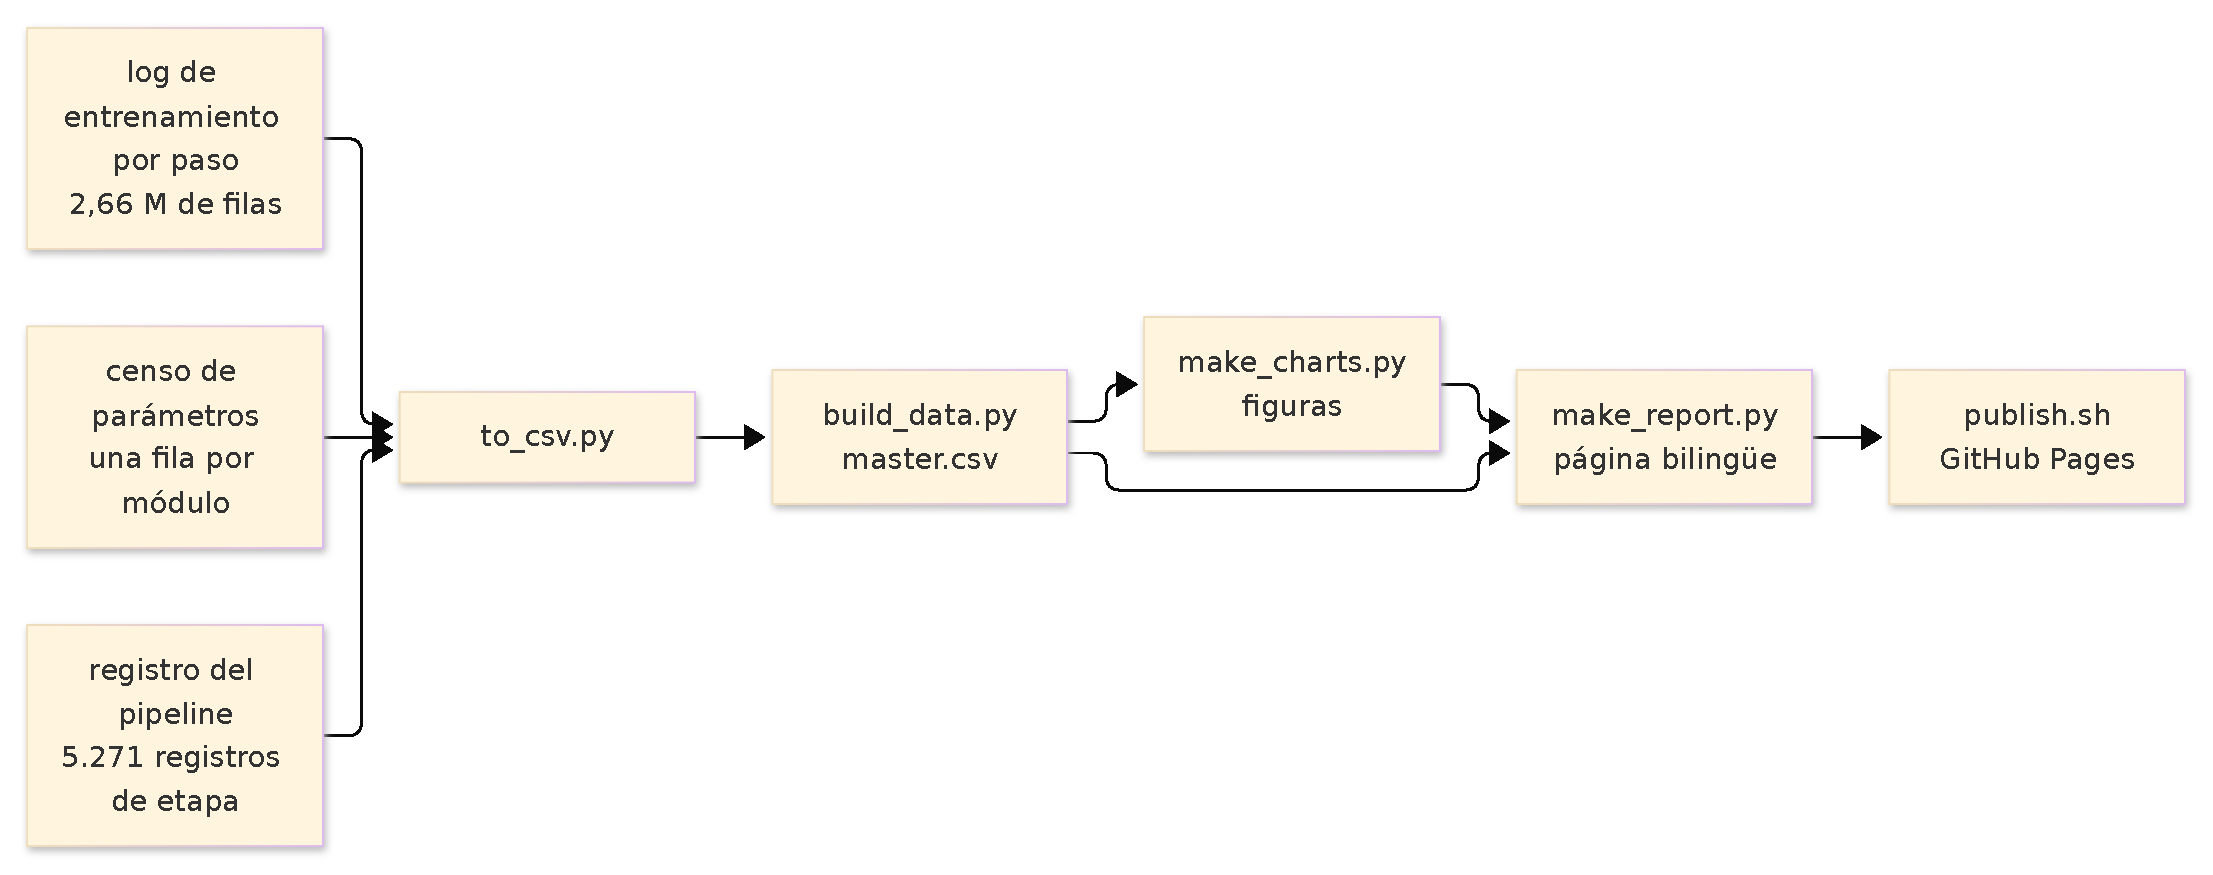
\includegraphics{../paper/figures/experiment-reporting-es.pdf}}
\caption{La cadena de reporte offline. Los tres registradores se consolidan en archivos CSV, se unen por configuración en \texttt{master.csv}, se grafican en ambos temas y se renderizan en una página estática bilingüe con los datasets unidos publicados al lado. Nada de esta cadena necesita GPU.}
\label{fig:experiment-reporting}
\end{figure}

\subsection{El libro de etapas de la ronda~2}

La Tabla~\ref{tab:stage-ledger} reproduce el libro. El entrenamiento domina tanto el conteo de registros como el coste: 1{,}039 intentos, de los cuales 868 tuvieron éxito y 171 fallaron, con una mediana de 68 minutos y un P90 de 84 minutos por intento---906 horas de CPU en total, de las cuales 905 corresponden a las 868 corridas analizadas y el resto a los intentos descartados. Todas las demás etapas se miden en segundos. El despliegue es la única etapa además del entrenamiento que falla (104 veces de 1{,}734), y los fallos son simétricos: siempre que el export estándar de una configuración falla, falla también su export cuantizado. La simetría apunta a una causa raíz compartida aguas arriba de la cuantización---la serialización del checkpoint o de la configuración---y no al paso de cuantizar en sí. La evaluación y el export a Hugging Face nunca fallaron en la población analizada.

\begin{table}[H]
\centering
\small
\caption{Libro de etapas del pipeline para la ronda~2. Las duraciones están en segundos; los totales son horas de reloj de toda la campaña.}
\label{tab:stage-ledger}
\begin{tabular}{lrrrrrr}
\toprule
Etapa & Registros & OK & Fallos & Mediana (s) & P90 (s) & Total (h) \\
\midrule
Entrenamiento          & 1{,}039 & 868  & 171 & 4{,}101,45 & 5{,}037,3 & 906,0 \\
Export a HF            & 867     & 867  & 0   & 17,41      & 44,7      & 5,4   \\
Evaluación de inferencia & 1{,}630 & 1{,}630 & 0 & 10,37     & 13,1      & 4,9   \\
Despliegue             & 1{,}734 & 1{,}630 & 104 & 8,64     & 38,0      & 8,8   \\
BitNet GGUF            & 1       & 1    & 0   & 3,32       & 3,3       & 0,0   \\
\bottomrule
\end{tabular}
\end{table}

Los 275 fallos son informativos y no un mero inconveniente. Los 171 fallos de entrenamiento quedan fuera de las 868 configuraciones analizadas, que se eligieron precisamente porque entrenaron; los 104 fallos de despliegue ocurren en pares simétricos, como se explicó arriba. Leído como medición de fiabilidad, el libro dice que el pipeline falla de forma ruidosa y temprana---en entrenamiento o en export---y nunca en silencio durante la evaluación. La distribución de fallos por familia y el análisis de huellas idénticas de los cuatro mezcladores que colapsan con 32 tokens se grafican en el Apéndice~\ref{sec:annex-experiment-2}.

\subsection{Datasets consolidados}

La cadena de reporte parte de las carpetas crudas por corrida y produce un conjunto pequeño de tablas unidas (Tabla~\ref{tab:round-datasets}). La clave de unión es el slug de configuración: \texttt{master.csv} lleva una fila por configuración con el censo de parámetros, el resumen de entrenamiento, los estados de etapa y las puntuaciones de inferencia uno al lado del otro. Las tablas se publican con el informe para que cualquier figura se pueda reconstruir sin los 702\,MB de logs paso a paso, y los CSV crudos por corrida se publican aparte, comprimidos con gzip, para quien necesite datos a nivel de paso.

\begin{table}[H]
\centering
\small
\caption{Archivos publicados con una ronda. \texttt{master.csv} es la clave de unión: una fila por configuración con parámetros, entrenamiento, pipeline e inferencia.}
\label{tab:round-datasets}
\begin{tabularx}{\linewidth}{L{5.2cm}L{9.4cm}}
\toprule
Archivo & Contenido \\
\midrule
\texttt{master.csv} & Una fila por configuración; parámetros por grupo, métricas de entrenamiento finales y promediadas, duraciones y estados de etapa, puntuaciones de inferencia por formato. \\
\texttt{training\_per\_epoch.csv} & Medias por corrida y época de pérdida, precisión, learning rate, normas de gradiente y rendimiento (2,66\,M de pasos reducidos a 86{,}274 filas). \\
\texttt{inference\_samples.csv} & Cada registro de inferencia: cuatro muestras, dos formatos, una fila por muestra. \\
\texttt{pipeline\_stages.csv} & El libro de etapas completo (5{,}271 filas). \\
\texttt{param\_metrics.csv} & El censo crudo de parámetros por grupo de módulos. \\
\texttt{training\_metrics\_avg.csv} & Promedios por corrida de las 34 métricas registradas. \\
\texttt{training\_metrics\_final.csv} & Instantánea del último paso de cada corrida. \\
\texttt{training\_metrics\_std.csv} & Desviaciones estándar muestrales por corrida. \\
\texttt{results.md.csv} & Resumen legible de los resultados del pipeline. \\
\texttt{data/raw/*.csv.gz} & Los 868 logs de paso por corrida, un archivo por configuración. \\
\bottomrule
\end{tabularx}
\end{table}

\subsection{Reconstruir una ronda}

El pipeline son tres scripts y un publicador, todos de biblioteca estándar o solo pandas/numpy/matplotlib, y todos ejecutan en CPU:

\begin{enumerate}[leftmargin=*]
    \item \texttt{python experimentos/to\_csv.py N} lee \texttt{experimentos/N/} sin modificarlo y escribe CSVs consolidados en \texttt{experimentos/N/csvs/}: la tabla de inferencia con la columna \texttt{notes} expandida en una columna por cada par \texttt{key=value}, el censo de parámetros como una fila por configuración, el libro de resultados como tabla plana, y los CSV de entrenamiento por corrida concatenados junto con su media, desviación estándar y última fila por corrida.
    \item \texttt{python experimentos/N/report/build\_data.py} procesa los logs crudos en streaming, une los tres registradores por slug y escribe \texttt{master.csv} y las tablas derivadas.
    \item \texttt{python experimentos/N/report/make\_charts.py} renderiza cada figura dos veces (tema oscuro y claro) y registra los pies en \texttt{registry.json}; \texttt{make\_report.py} consume ambos para emitir la página estática bilingüe.
    \item \texttt{bash experimentos/N/report/publish.sh} copia la página, las figuras y los datasets al espejo de GitHub Pages. Nunca hace commit ni push por sí mismo.
\end{enumerate}

Las figuras del artículo son un subconjunto curado de los mismos constructores de gráficos, exportado como PDF vectorial por \texttt{make\_paper\_figures.py}. La división del trabajo es deliberada: un mismo conjunto de constructores alimenta el informe web y el artículo, así que un número del artículo y el píxel correspondiente del sitio no pueden divergir. Toda la cadena es solo CPU y reproduce cada número de este apéndice a partir de los datasets publicados.

\subsection{Ronda 1: el piloto}

La ronda~1 ejercitó el mismo arnés de extremo a extremo a escala de humo: 5{,}129 registros de etapas, corridas de entrenamiento de aproximadamente medio minuto y la misma secuencia de cinco etapas. Su propósito era validar la mecánica---la generación de slugs, la contabilidad del libro, la simetría del despliegue y las uniones del reporte---antes de comprometer tiempo de CPU en la campaña real. No se analiza más aquí porque las corridas eran demasiado cortas para separar arquitecturas; su valor es procedimental: la ronda~2 heredó un arnés cuya contabilidad ya estaba ejercitada y cuyos modos de fallo ya eran conocidos.
